\begin{figure*}[!ht]
    \centering
    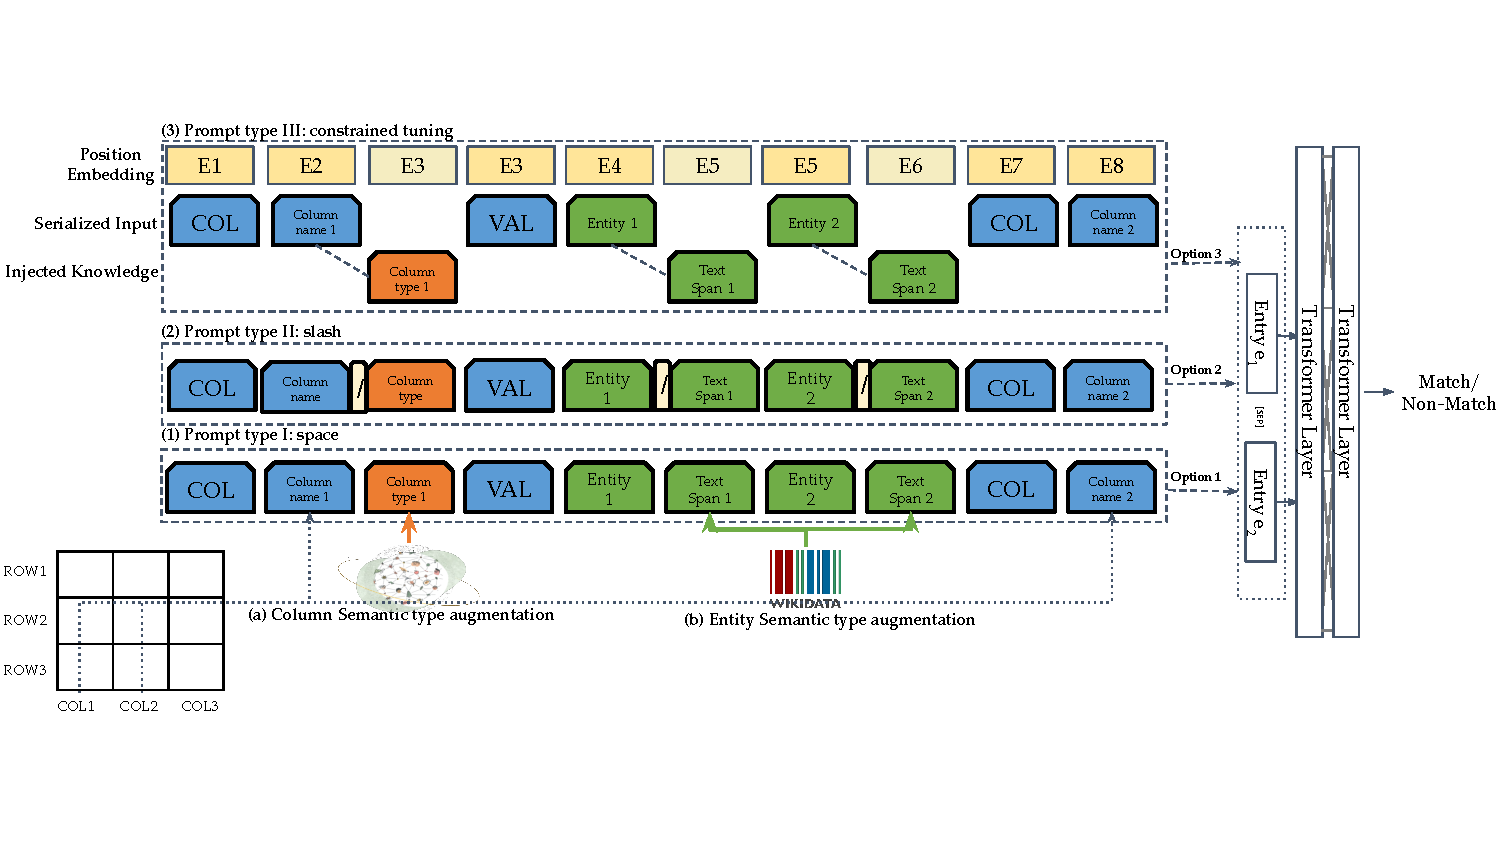
\includegraphics[width=\linewidth]{plots/DCER_short.pdf}
    \vspace{-0.8cm}
    \caption{The framework of KAER. First, (a)column semantic type augmentation and (b)entity semantic type augmentation are used to inject domain knowledge from both column and entity levels of the input table. 
    Then three options of prompting types are provided after external knowledge injection: (1) using space; (2) using ``/''; (3) using additional position encoding. 
    With the knowledge injection and prompting methods, the serialized sequence is fed into the PLMs.}
    \vspace{-0.5cm}
    \label{fig:framework}
\end{figure*}

% \subsection{Data Preparation: a Preceding Stage of Entity Resolution}

% Data quality impacts the cost and performance of entity resolution systems significantly. Even for an error-free system with perfectly clean data, data from multiple sources are often not saved in a consistent way or carefully controlled for quality \cite{elmagarmid_duplicate_2007}. Usually, the data preparation stage includes parsing, data transformation, and standardization steps, and the goal is to improve the quality of the in-flow data and make the data comparable, and more usable \cite{elmagarmid_duplicate_2007}. 

% Even though adjusting and selecting data preparators to prepare data before doing the entity resolution is not the focus of this paper, we will still apply some general data transformations to deal with specific data types. Data transformations are used to convert the data into the correct type or format that conforms to their domains \cite{elmagarmid_duplicate_2007}. Enhancing data quality by preprocessing data also contributes to the result of Sherlock \cite{hulsebos_sherlock_2019}, which can detect the semantic data types. Here we mainly use general transformations to help normalize the atomic types of data, such as \textit{string}, \textit{integer}, \textit{Boolean}. For instance, the \textit{float} type of data values for $Year$ is meaningless. So a simple conversion of the data from \textit{float} to \textit{integer} is required. Meanwhile, encoding issues also appear across the data values that need to be addressed at this stage. For numerical data, range checking could be used to ensure that data is in the appropriate range \cite{elmagarmid_duplicate_2007}. Preprocessing composite data values will be more complicated that requires a few steps, i.e., we usually first split the data values and then prepare data values separately, and finally merge the cleaned data values.

% \subsection{Schema Matching: The Context of Entity Resolution}
% % Assigned to Lan Li
% Entity resolution is to identify and match records that refer to the same real-world entity. In many situations, raw records are stored from heterogeneous sources, while most existing techniques on entity resolution predefine the same schema for records from different sources \cite{elmagarmid_duplicate_2007}. Moreover, records from different sources might follow different structures at the attribute level, which adds more difficulties for entity resolution tasks \cite{enriquez_entity_2017, arabnia_when_2021}. Therefore, schema matching is required to discuss before we talk about entity resolution tasks. In particular, we consider the schema matching task as the context of processing entity resolution for schema matching guides which two records should be paired at the column level before processing the entity resolution at the row level. \cite{lin_efficient_2020} perform schema matching by creating a \textit{full schema} in which they compare and merge records from different sources into \textit{super record} before the entity resolution. In this way, they avoid information loss during the schema-matching process.

% The main operation in manipulating schema information is \textit{Match}, which inputs two schemas and produces a mapping between two elements of the two schemas that relate semantically to each other \cite{rahm_survey_2001}. \cite{rahm_survey_2001} select the matching algorithms (a.k.a matchers) based on the application domain and schema types, and use data types to constrain the search space of correspondences. 

\subsection{Pretrained Model for Entity Resolution}
% Assigned to Lan Li

% \cite{zhao_auto-em_2019} propose a transfer-learning approach to entity matching (EM), leveraging pre-trained entity matching models that are based on large-scale, production knowledge bases (KB). Auto-EM enables entity type detection and entity matching at the attribute level by learning a large amount of data from KBs. In this way, they achieve a high EM quality with little labeled training data. \cite{wu_zeroer_2020} introduce ZeroER that requires \textit{Zero} labeled examples for entity resolution task. They leverage a powerful generative model based on Gaussian Mixture Models for learning the match and mismatch distributions. 

% Unlike Recurrent Neural Network (RNN) used in \cite{zhao_auto-em_2019, mudgal_deep_2018}, 
A few recent works apply transformer-based PLMs to entity resolution tasks. \citet{paganelli_analyzing_2022} discover that simply fine-tuning BERT can benefit matching/non-matching classification tasks and BERT can recognize the input sequence as a pair of records. \citet{li_improving_2021} leverage siamese network structure with PLMs to improve the efficiency of PLMs during the blocking phase. 
Ditto by \cite{li_deep_2020} is now the state-of-the-art entity matching system based on PLMs, i.e., RoBERTa. In addition, Ditto provides a deeper language understanding for entity resolution by injecting domain knowledge, summarizing the key information, and augmenting with more difficult examples for training data. 
% Ditto injects dataset type and numeric data type as the domain knowledge. Inspired by ditto, we aim to corporate column type semantic and e
 
% Auto-EM introduce the framework to pretrain an RNN-based attribute type classifier on large knowledge base .
\vspace{-0.5em}
\subsection{Knowledge Augmentation}
Recent works show that injecting external knowledge to PLMs can benefit Natural Language Reprocessing (NLP) downstream tasks~\cite{zhang_ernie_2019,peters_knowledge_2019,liu_k-bert_2020,wang_k-adapter_2021, wang_kepler_2021}. 
Recent studies on semantic column type augmentation and entity linking can inject external domain knowledge into PLMs at the schema and entity levels. 
Semantic column-type augmentation can inject domain-specific knowledge for columns with/without existing column names. Existing studies~\cite{hulsebos_sherlock_2019,suhara_annotating_2022} use deep learning approaches to detect semantic data types at the column level.
% Sherlock \cite{hulsebos_sherlock_2019} is a novel system that uses a deep learning approach to detect semantic data types at the column level. 
% Sherlock predicts the conceptual domain of a column when there is no schema or the existing schema cannot provide a fine-grained description of the data.
% Doduo~\cite{suhara_annotating_2022} is another recent method for annotating  columns with semantic types and for adding semantic relations between columns. 
% % \subsubsection{Entity linking}
In addition, entity linking \cite{li_deep_2020} refers to the task of linking entity mentions appearing in natural language text with their corresponding entities in an external knowledge base, e.g., Wikidata. 
% Existing study has explored using PLMs to perform entity linking tasks, and achieved promising results. 
% \citet{zhang_ernie_2019} introduced the model ERNIE by jointly pre-training BERT with a masked language modeling objective. The knowledge augmented BERT model is found to outperform existing methods in multiple knowledge-driven tasks. 
% Later work by \citet{peters_knowledge_2019} futher improved the ERNIE model by introducing a trainable entity linker module and alignment between entity embedding and BERT embedding. 
Recent work by \citet{ayoola_refined_2022} introduces an entity linking method by fine-tuning a PLM over Wikipedia data, which we use as the method for entity linking in our study. 

% \subsubsection{Knowledge prompting} %\liri{Liri}
The method of conditioning the language model, a.k.a, ``prompting'', is a hot topic in Nature Language Processing \citet{pengfeiliu}. \citet{kojima_large_2022} propose Zero-shot-CoT, a single zero-shot prompt that evokes a chain of thought from large language models, highlighting that the performance of the language model has been affected by different templates of the prompt.
Furthermore, the method to inject the identified external knowledge into PLMs matters. \citet{liu_k-bert_2020} propose the model K-BERT adding soft-position encoding and visible matrix to the augmented input sequence to reduce knowledge noise injected into the original input and corresponding models. 
%Another direction of knowledge incorporation is to align the knowledge embedding and PLMs output into same embedding space. The work from Wang et al. \cite{wang_kepler_2021} introduced a joint pre-training method based on RoBERTa to map knowledge base entity and natural language entity description into the sample space. The knowledge embedding produced by KEPLER can be utilized as an additional input information source in our entity resolution task. The effectiveness of these methods in incorporating knowledge into entity resolution tasks can be further explored.

